\documentclass[tikz,border=1pt]{standalone} 

\usepackage[utf8]{inputenc}
\usepackage{tikz}
\usepackage{amsmath}
\usetikzlibrary{positioning, arrows.meta} 
\usepackage{microtype}
\usepackage{graphicx}
\usepackage{caption}
\usepackage{booktabs} 
\usepackage{enumitem} 
\usepackage{pgfplots} 
\pgfplotsset{compat=1.17}  
\usepackage{tikz-cd} 
\usepackage{wrapfig} 
\usepackage{tkz-euclide} 
\usetikzlibrary{decorations.pathreplacing} 
\usepackage{xr}
\externaldocument{main} 
\usepackage{hyperref}
\usepackage[capitalize,noabbrev]{cleveref}

\begin{document}
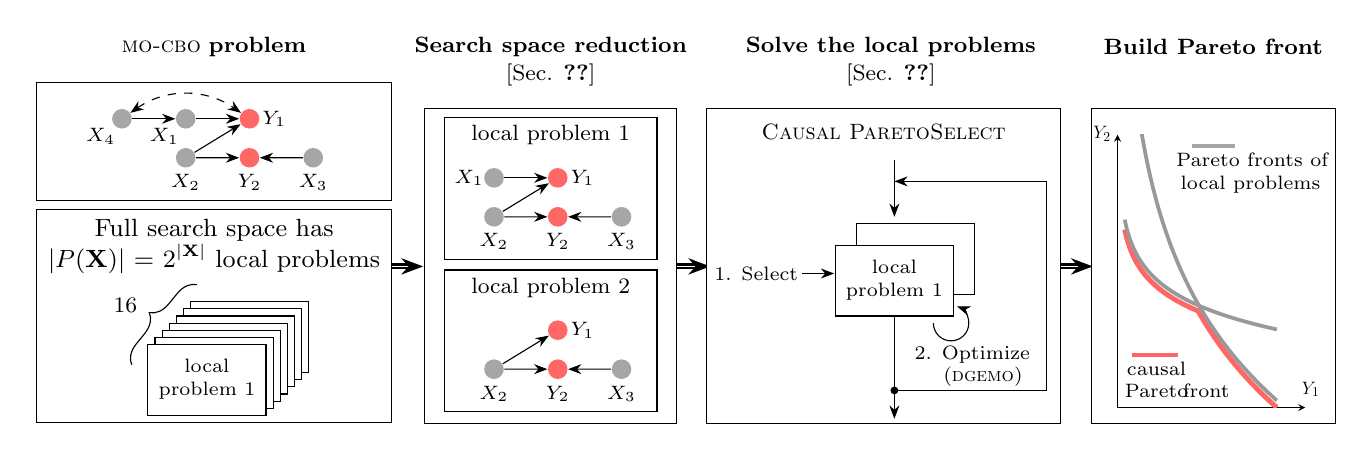
\begin{tikzpicture}[scale=0.45,
    ->, 
     >=Stealth, 
    every edge/.style={draw}, 
    box/.style={draw, fill=white,
                minimum width=2.4cm,
                minimum height=1.5cm
                },
    ellipsis/.style={font=\large}
    ovbx/.pic={\foreach \c in {0,.1,.2}
                    \node[box] (X\c) at (\c,-\c) {};
                \coordinate (-WE) at (X0.west);
              },
    ]

    \node[font=\footnotesize] at (5,-0.8) {\textsc{mo-cbo} \textbf{problem}};
    \node[font=\footnotesize] at (14.5,-0.8) {\textbf{Search space reduction}};
    \node[font=\footnotesize] at (14.5,-1.6) {[Sec. \ref{subsec:search_space_reduction}]};
    \node[font=\footnotesize] at (24.1,-0.8) {\textbf{Solve the local problems}};
    \node[font=\footnotesize] at (24.1,-1.6) {[Sec. \ref{subsec:mo_cbo_algorithm}]};
    \node[font=\footnotesize] at (33.2,-0.8) {\textbf{Build Pareto front}};

    \draw[double,thick] (10.0,-7) -- (10.9,-7); 
    \draw[double,thick] (18.0,-7) -- (19.0,-7); 
    \draw[double,thick] (28.9,-7) -- (29.8,-7); 

    \node[draw, minimum width=4.5cm, minimum height=1.5cm, outer sep=0, anchor=north west] (main_problems_box) at (0, -1.8) {};
    
    \begin{scope}[shift={(main_problems_box.south)}, xshift=1.0cm, yshift=6.8cm]
        \node[circle, inner sep=2.5pt, fill=gray!70] (X4) at (-3.6, -4.5) {};
        \node[font=\scriptsize] (X4_ann) at (-4.2, -5.0) {$X_4$};
        \node[circle, inner sep=2.5pt, fill=gray!70] (X1) at (-1.8, -4.5) {};
        \node[font=\scriptsize] (X1_ann) at (-2.4, -5.0) {$X_1$};
        \node[circle, inner sep=2.5pt, fill=gray!70] (X2) at (-1.8, -5.6) {};
        \node[font=\scriptsize] (X2_ann) at (-1.8, -6.3) {$X_2$};
        \node[circle, inner sep=2.5pt,fill=red!60] (Y1) at (0.0, -4.5) {};
        \node[font=\scriptsize] (Y1_ann) at (0.7, -4.5) {$Y_1$};
        \node[circle, inner sep=2.5pt, fill=red!60] (Y2) at (0.0, -5.6) {};
        \node[font=\scriptsize] (Y2_ann) at (0.0, -6.3) {$Y_2$};
        \node[circle, inner sep=2.5pt,  fill=gray!70] (X3) at (1.8, -5.6) {};
        \node[font=\scriptsize] (X3_ann) at (1.8, -6.3) {$X_3$};
        \draw (X1) edge (Y1);
        \draw (X2) edge (Y1);
        \draw (X2) edge (Y2);
        \draw (X3) edge (Y2);
        \draw (X4) edge (X1);
        \draw[dashed, <->, bend left=35] (X4) to (Y1);
    \end{scope}

    \node[draw, minimum width=4.5cm, minimum height=2.7cm, outer sep=0, anchor=north west] (local_problems_box) at (0, -5.4) {};

    \node[align=center, font=\small, anchor=north, text width=4.5cm] at (local_problems_box.north) {Full search space has $|\mathbb{P}(\mathbf{X})| = 2^{|\mathbf{X}|}$ local problems};

    \begin{scope}[shift={(local_problems_box.south)}, xshift=1.0cm, yshift=2.4cm] 
        \node[draw, fill=white, minimum width=1.5cm, minimum height=0.9cm] at (0,0) {};
        \node[draw, fill=white, minimum width=1.5cm, minimum height=0.9cm] at (-0.2,-0.2) {};
        \node[draw, fill=white, minimum width=1.5cm, minimum height=0.9cm] at (-0.4,-0.4) {};
        \node[draw, fill=white, minimum width=1.5cm, minimum height=0.9cm] at (-0.6,-0.6) {};
        \node[draw, fill=white, minimum width=1.5cm, minimum height=0.9cm] at (-0.8,-0.8) {};
        \node[draw, fill=white, minimum width=1.5cm, minimum height=0.9cm] at (-1.0,-1.0) {};
        \node[draw, fill=white, minimum width=1.5cm, minimum height=0.9cm] at (-1.2,-1.2) {};

        \node[font=\scriptsize] at (-1.2,-0.8) {local};
        \node[font=\scriptsize] at (-1.2,-1.5) {problem 1};
        \draw[-,decorate, decoration={brace, amplitude=7pt}, rotate=135] (1.8,2.9) -- (2.1,-0.0); 
        \node[font=\footnotesize] at (-3.5,0.9) {16};
    \end{scope}
    

    \node[box, minimum width=3.2cm, minimum height=4cm] at (14.5, -7) {};
    \node[box, minimum width=2.7cm, minimum height=1.8cm] at (14.5, -4.8) {};
    \node[font=\footnotesize] at (14.5,-3.3) {local problem 1};
    \node[circle, inner sep=2.5pt, fill=gray!70] (X1) at (12.9, -4.5) {};
    \node[font=\scriptsize] (X1_ann) at (12.2, -4.5) {$X_1$};
    \node[circle, inner sep=2.5pt, fill=gray!70] (X2) at (12.9, -5.6) {};
    \node[font=\scriptsize] (X2_ann) at (12.9, -6.3) {$X_2$};
    \node[circle, inner sep=2.5pt,fill=red!60] (Y1) at (14.7, -4.5) {};
    \node[font=\scriptsize] (Y1_ann) at (15.4, -4.5) {$Y_1$};
    \node[circle, inner sep=2.5pt, fill=red!60] (Y2) at (14.7, -5.6) {};
    \node[font=\scriptsize] (Y2_ann) at (14.7, -6.3) {$Y_2$};
    \node[circle, inner sep=2.5pt,  fill=gray!70] (X3) at (16.5, -5.6) {};
    \node[font=\scriptsize] (X3_ann) at (16.5, -6.3) {$X_3$};
    \draw (X1) edge (Y1);
    \draw (X2) edge (Y1);
    \draw (X2) edge (Y2);
    \draw (X3) edge (Y2);

    \node[box, minimum width=2.7cm, minimum height=1.8cm] at (14.5, -9.1) {};
    \node[font=\footnotesize] at (14.5,-7.6) {local problem 2};
    \node[circle, inner sep=2.5pt, fill=gray!70] (X2) at (12.9, -9.9) {};
    \node[font=\scriptsize] (X2_ann) at (12.9, -10.6) {$X_2$};
    \node[circle, inner sep=2.5pt,fill=red!60] (Y1) at (14.7, -8.8) {};
    \node[font=\scriptsize] (Y1_ann) at (15.4, -8.8) {$Y_1$};
    \node[circle, inner sep=2.5pt, fill=red!60] (Y2) at (14.7, -9.9) {};
    \node[font=\scriptsize] (Y2_ann) at (14.7, -10.6) {$Y_2$};
    \node[circle, inner sep=2.5pt,  fill=gray!70] (X3) at (16.5, -9.9) {};
    \node[font=\scriptsize] (X3_ann) at (16.5, -10.6) {$X_3$};
    \draw (X2) edge (Y1);
    \draw (X2) edge (Y2);
    \draw (X3) edge (Y2);


    \node[box, minimum width=4.5cm, minimum height=4cm] at (23.9, -7) {};
    \node[font=\footnotesize] at (23.9, -3.2) {\textsc{Causal ParetoSelect}};
    \node[box, minimum width=1.5cm, minimum height=0.9cm] at (24.8, -6.8) {};
    \node[box, minimum width=1.5cm, minimum height=0.9cm] at (24.2, -7.4) {};
        % Text
    \node[font=\scriptsize] at (24.2,-7) {local};
    \node[font=\scriptsize] at (24.2,-7.7) {problem 1};
    \node[font=\scriptsize] at (20.3, -7.2) {1. Select};
    \node[font=\scriptsize] at (26.4, -9.5) {2. Optimize};
    \node[font=\scriptsize] at (26.7, -10.1) {(\textsc{dgemo})};
    \draw[->] (21.6,-7.2) -- (22.5,-7.2); 
    \draw[->] (25.3,-8.6) arc[start angle=180, end angle=430, radius=0.5cm]; 
    \draw[->] (24.2,-4) -- (24.2,-5.6);   
    \draw[->] (28.5,-4.6) -- (24.2,-4.6); 
    \draw[-] (28.5,-4.6) -- (28.5,-10.5); 
    \draw[->] (24.2,-8.4) -- (24.2,-11.3);
    \draw[-] (28.5,-10.5) -- (24.2,-10.5); 
    \node[circle,fill=black,inner sep=1] at (24.2,-10.5) {};


    \node[box, minimum width=3.1cm, minimum height=4cm] at (33.2, -7) {};
    \draw[-,ultra thick, red!60] (30.9, -9.5) -- (32.2, -9.5);
    \node[font=\scriptsize] at (31.6, -9.9) {causal};
    \node[font=\scriptsize] at (31.6, -10.5) {Pareto};
    \node[font=\scriptsize] at (33.0, -10.5) {front};
    \draw[-,ultra thick, gray!70] (32.6, -3.6) -- (33.8, -3.6);
    \node[font=\scriptsize] at (34.3, -4.0) {Pareto fronts of};
    \node[font=\scriptsize] at (34.25, -4.7) {local problems};

    \begin{axis}[
        scale only axis,
        no markers,
        domain=0:5,
        samples=100,
        axis lines=center,
        axis line style={line width=1.5pt},
        ticks=none,
        xmin=0, xmax=5.3,            
        ymin=, ymax=10,   
        xlabel={$Y_1$},
        ylabel={$Y_2$},
        xlabel style={yshift=5pt, xshift=15pt, font=\fontsize{15}{17}\selectfont},
        ylabel style={yshift=10pt, xshift=-23pt, font=\fontsize{15}{17}\selectfont},
        height=7.7cm,                  % Set the height of the plot
        width=5.3cm,
        at={(3050,-110)}]
        \addplot[red!60, -, line width=4pt, restrict x to domain=0.2:2.35] {5.8 - 0.95*ln(x)}; 
        \addplot[red!60, -, line width=4pt, restrict x to domain=2.25:4.5] {8.3 - 4*ln(x)}; 
        \addplot[gray!80, -, thick, line width=3pt, restrict x to domain=0.2:4.5] {8.5 - 4*ln(x)};  
        \addplot[gray!80, -, thick, line width=3pt, restrict x to domain=0.2:4.5] {6 - ln(x)};
    \end{axis}
    \vspace{-0.2cm}
\end{tikzpicture}
\end{document}